\section{Results}
\label{sec:results}

\subsection{Heterogeneity}
\label{sec:heterogeneity}

\Cref{tab:performance} is the performance matrix. Blank primitive--task pairs were not eligible. Missing primitive--task pairs are left blank rather than assigned zero. Cfull and C100k are the classifier. Device is part of the record.

\begin{table}[htbp]
\centering
\footnotesize
\setlength{\tabcolsep}{3.2pt}
\caption{Measured profiles. \(Q\) is macro-F1. Train and infer are seconds. API cost is zero because no API was called. Latency is milliseconds and does not include model load. Invalid is a count. The rule, classifier, and Laya were run on CPU. Qwen was run on a GTX 1650 Ti in float16. C100k marks the pre-registered 100{,}000-row classifier fit. Source: \protect\path{research/docs/performance_matrix.md}.}
\label{tab:performance}
\begin{tabular}{@{}llrrrrrrrrr@{}}
\toprule
& & & \multicolumn{2}{c}{Time (s)} & & \multicolumn{2}{c}{Latency (ms)} & & & \\
\cmidrule(lr){4-5}\cmidrule(lr){7-8}
Task & Primitive & \(Q\) & Train & Infer & API (\$) & p50 & p95 & Invalid & \(n\) & Device \\
\midrule
SMS Spam & Rule & 0.8576 & 0.000 & 0.028 & 0 & 0.020 & 0.062 & 0 & 1000 & CPU \\
SMS Spam & Classifier & 0.9393 & 0.295 & 0.351 & 0 & 0.188 & 0.719 & 0 & 1000 & CPU \\
SMS Spam & Laya & 0.7822 & 0.000 & 724.349 & 0 & 698.724 & 941.798 & 0 & 1000 & CPU \\
SMS Spam & Qwen & 0.2067 & 0.000 & 308.276 & 0 & 323.515 & 417.066 & 25 & 1000 & GPU \\
PubMedQA & Classifier & 0.2691 & 0.635 & 0.194 & 0 & 0.261 & 0.623 & 0 & 500 & CPU \\
PubMedQA & Laya & 0.3128 & 0.000 & 1019.183 & 0 & 1978.849 & 2842.361 & 0 & 500 & CPU \\
PubMedQA & Qwen & 0.2327 & 0.000 & 474.746 & 0 & 932.252 & 1239.578 & 174 & 500 & GPU \\
Banking77 & Classifier & 0.8508 & 2.412 & 0.267 & 0 & 0.184 & 0.456 & 0 & 1000 & CPU \\
Banking77 & Laya & 0.3888 & 0.000 & 5260.039 & 0 & 5212.193 & 5888.881 & 0 & 1000 & CPU \\
Banking77 & Qwen & 0.1316 & 0.000 & 1360.532 & 0 & 1274.864 & 1668.698 & 514 & 1000 & GPU \\
CLINC150 plus & Classifier & 0.8299 & 5.033 & 0.237 & 0 & 0.177 & 0.337 & 0 & 1000 & CPU \\
CLINC150 plus & Laya & 0.4280 & 0.000 & 4614.129 & 0 & 4584.007 & 4905.017 & 0 & 1000 & CPU \\
CLINC150 plus & Qwen & 0.2465 & 0.000 & 1455.811 & 0 & 1336.641 & 1980.492 & 745 & 1000 & GPU \\
LEDGAR & Classifier & 0.7418 & 139.867 & 0.298 & 0 & 0.215 & 0.481 & 0 & 1000 & CPU \\
LEDGAR & Laya & 0.2088 & 0.000 & 4724.659 & 0 & 4528.972 & 6190.025 & 0 & 1000 & CPU \\
LEDGAR & Qwen & 0.0281 & 0.000 & 1346.729 & 0 & 1236.580 & 1887.759 & 86 & 1000 & GPU \\
Civil Comments & Classifier (C100k) & 0.6298 & 19.757 & 0.316 & 0 & 0.196 & 0.628 & 0 & 1000 & CPU \\
Civil Comments & Laya & 0.7367 & 0.000 & 807.656 & 0 & 726.485 & 1376.470 & 0 & 1000 & CPU \\
Civil Comments & Qwen & 0.0000 & 0.000 & 544.926 & 0 & 489.657 & 808.857 & 1000 & 1000 & GPU \\
VitaminC & Classifier (C100k) & 0.3826 & 15.300 & 0.251 & 0 & 0.176 & 0.416 & 0 & 1000 & CPU \\
VitaminC & Laya & 0.2165 & 0.000 & 797.699 & 0 & 766.750 & 1045.356 & 0 & 1000 & CPU \\
VitaminC & Qwen & 0.2209 & 0.000 & 603.543 & 0 & 578.279 & 779.076 & 23 & 1000 & GPU \\
ESCI & Classifier (C100k) & 0.2189 & 77.896 & 0.253 & 0 & 0.181 & 0.394 & 0 & 1000 & CPU \\
ESCI & Laya & 0.1527 & 0.000 & 1909.519 & 0 & 1444.679 & 4742.117 & 0 & 1000 & CPU \\
ESCI & Qwen & 0.0358 & 0.000 & 1024.658 & 0 & 922.247 & 2060.757 & 32 & 1000 & GPU \\
\bottomrule
\end{tabular}
\end{table}

\begin{table}[htbp]
\centering
\small
\caption{Qwen invalid-output rate. Rate is the invalid count divided by the evaluation count \(n\). The rule, the classifier, and Laya have zero invalid outputs on every scored task.}
\label{tab:validity}
\begin{tabular}{@{}lrr@{}}
\toprule
Task & Invalid / \(n\) & Rate \\
\midrule
VitaminC & 23 / 1000 & 0.023 \\
SMS Spam & 25 / 1000 & 0.025 \\
ESCI & 32 / 1000 & 0.032 \\
LEDGAR & 86 / 1000 & 0.086 \\
PubMedQA & 174 / 500 & 0.348 \\
Banking77 & 514 / 1000 & 0.514 \\
CLINC150 plus & 745 / 1000 & 0.745 \\
Civil Comments & 1000 / 1000 & 1.000 \\
\bottomrule
\end{tabular}
\end{table}

\FloatBarrier

Macro-F1 on SMS Spam runs from 0.2067 (Qwen) to 0.9393 (classifier), with the rule at 0.8576 and Laya at 0.7822. On Banking77 the classifier reaches 0.8508 and Qwen 0.1316. On LEDGAR the classifier reaches 0.7418 and Qwen 0.0281. The relative ordering therefore varies across tasks. On PubMedQA, Laya's macro-F1 is 0.3128 and the classifier's is 0.2691. On Civil Comments, Laya's is 0.7367 and the C100k classifier's is 0.6298. On VitaminC, the classifier (0.3826) is ahead of Qwen (0.2209) and Laya (0.2165), and Qwen's invalid-output rate is only 0.023. The remaining performance gap is therefore largely attributable to the correctness of legal label predictions rather than output validity. The measurements are not collapsed into a single ranking.

Local inference time and latency are not comparable across devices. Classifier p50 latency is under 0.3\,ms on every task. Laya's p50 on CPU runs from 698.7\,ms on SMS Spam to 5212\,ms on Banking77. Qwen's p50 on the GTX 1650 Ti runs from 323.5\,ms on SMS Spam to 1336.6\,ms on CLINC150 plus. These values characterize the specific deployments used in this study. They do not establish intrinsic speed differences among the primitives. API cost does not vary.

\begin{figure}[htbp]
\centering
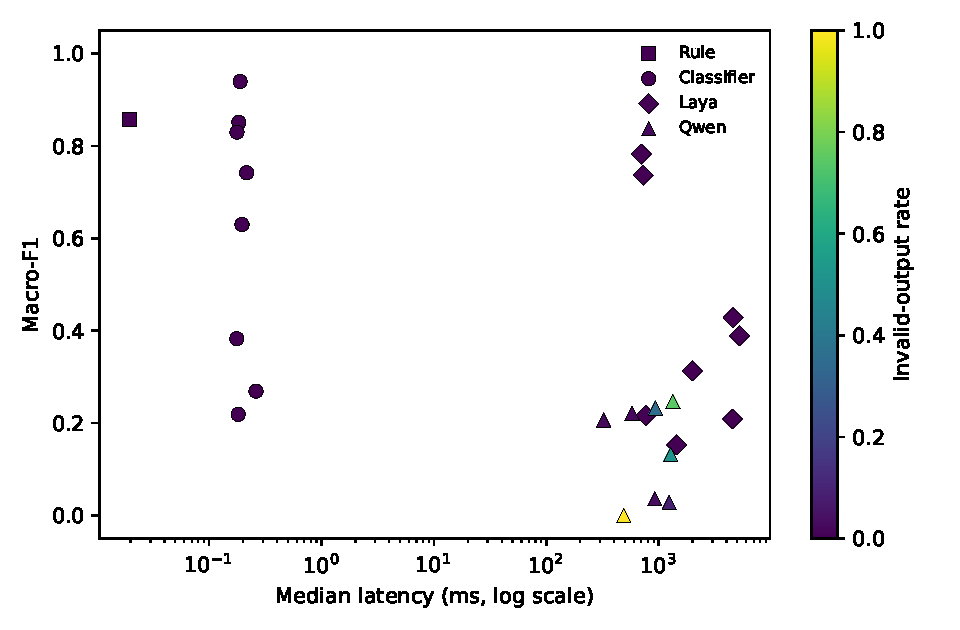
\includegraphics[width=\linewidth]{figures/figure2_heterogeneity.pdf}
\caption{Measured macro-F1 against p50 latency on a log scale, one marker per eligible pair in \cref{tab:performance}. Marker shape is the primitive. Color is the invalid-output rate. The rule, the classifier, and Laya are CPU timings. Qwen is the GTX 1650 Ti in float16. No trend line or confidence band is shown. Because the primitives were measured on different devices, latency should not be interpreted as a hardware-normalized comparison.}
\label{fig:latency-quality}
\end{figure}
\FloatBarrier

Training time is nonzero only for the classifier, from 0.295\,s on SMS Spam to 139.867\,s on LEDGAR. The C100k fits are 19.757\,s (Civil Comments), 15.300\,s (VitaminC), and 77.896\,s (ESCI).

\subsection{Prediction against the primitive mean}
\label{sec:prediction}

\Cref{tab:selector} is the task-level mean absolute error. Each cell averages the eligible primitives both predictors could fill. For the security holdout that set excludes the rule.

\begin{table}[htbp]
\centering
\small
\setlength{\tabcolsep}{5pt}
\caption{Held-out absolute error, ridge versus the training-fold primitive mean. Each cell averages the eligible primitives both predictors could fill. For the security holdout that set excludes the rule. The underlying numerical artifact is provided with the accompanying repository.}
\label{tab:selector}
\begin{tabular}{@{}llrrrr@{}}
\toprule
Holdout & Task & \(Q\) ridge & \(Q\) mean & \(V\) ridge & \(V\) mean \\
\midrule
Intent & Banking77 & 0.2112 & 0.1090 & 0.1713 & 0.0725 \\
Intent & CLINC150 plus & 0.1623 & 0.1232 & 0.2483 & 0.1495 \\
Verification & PubMedQA & 0.2583 & 0.2785 & 0.0792 & 0.0420 \\
Verification & VitaminC & 0.2096 & 0.2688 & 0.2839 & 0.1503 \\
Moderation & Civil Comments & 0.2075 & 0.1880 & 0.3333 & 0.2366 \\
Security & SMS Spam & 0.2271 & 0.2619 & 0.2832 & 0.1426 \\
Business / legal & LEDGAR & 0.1562 & 0.1684 & 0.1131 & 0.1188 \\
E-commerce & ESCI & 0.1024 & 0.2825 & 0.0444 & 0.1199 \\
\bottomrule
\end{tabular}
\end{table}


Ridge is closer on macro-F1 for PubMedQA, VitaminC, SMS Spam, LEDGAR, and ESCI. It is farther on Banking77, CLINC150 plus, and Civil Comments. Ridge is closer on the invalid-output rate only for LEDGAR and ESCI.

\begin{figure}[htbp]
\centering
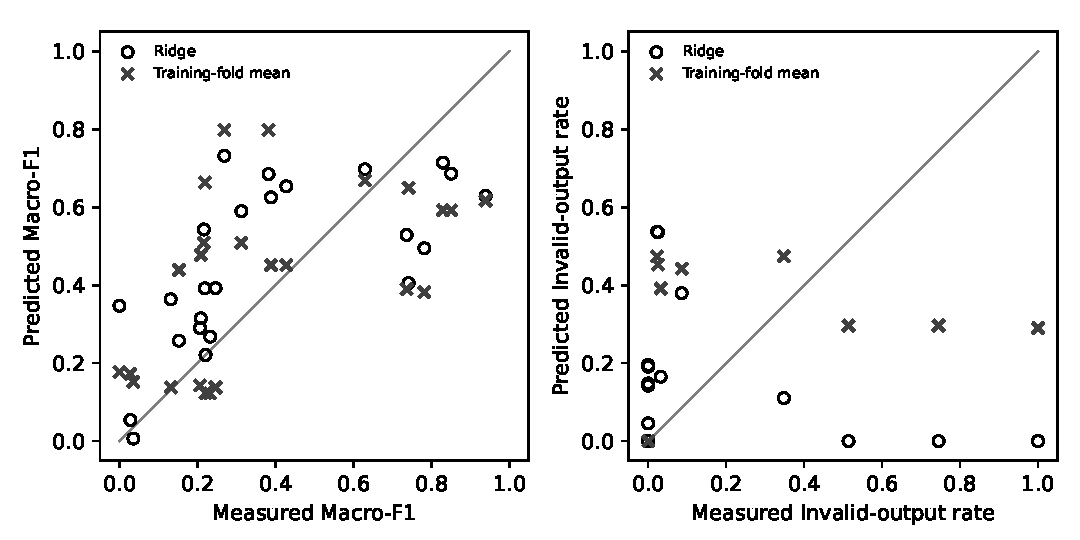
\includegraphics[width=\linewidth]{figures/figure3_prediction.pdf}
\caption{Predicted versus measured macro-F1, and predicted versus measured invalid-output rate, for held-out pairs both predictors filled. The diagonal is equality. Open circles are ridge. Crosses are the training-fold mean.}
\label{fig:prediction}
\end{figure}
\FloatBarrier

\begin{samepage}
p50-latency error is smaller for ridge on four tasks and smaller for the mean on four. Those errors are hundreds of milliseconds. They are reported in the result file and are not a hardware-normalized comparison. API-cost error is 0 for both predictors on every task, because every measured value is 0. That tie is not evidence of predictive skill.
\par
\end{samepage}

\begin{figure}[htbp]
\centering
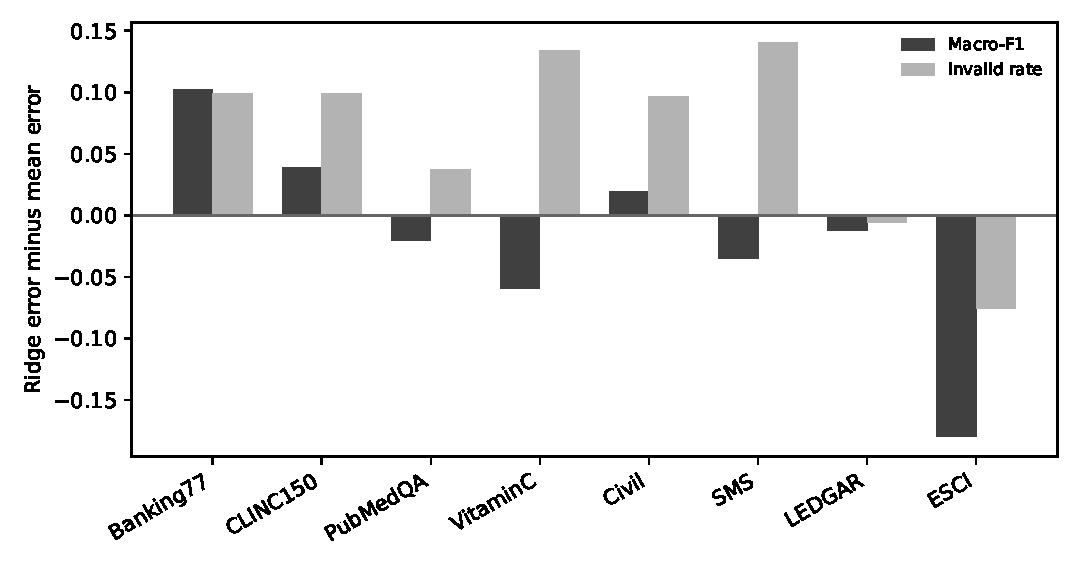
\includegraphics[width=\linewidth]{figures/figure4_error_difference.pdf}
\caption{Ridge absolute error minus training-fold-mean absolute error, for macro-F1 and for the invalid-output rate. A negative bar means ridge was closer; the differences are descriptive rather than inferential.}
\label{fig:error-difference}
\end{figure}
\FloatBarrier

On the fit that uses all seven selector-training tasks, the largest macro-F1 coefficients are the primitive indicators: Qwen \(-0.385\) and Laya \(-0.134\), against an intercept of 0.593. The largest fingerprint coefficient on that coordinate is normalized entropy, \(-0.065\). On the invalid-output rate, the Qwen indicator is \(+0.306\) and the largest fingerprint coefficient is mean label cosine, \(+0.113\). The fingerprint enters as a shift applied to every primitive. Invalid outputs in this matrix occur for Qwen. A shared shift cannot raise Qwen's invalid-output rate on a particular kind of task without also raising the classifier and Laya, whose invalid-output rates are 0.

The three largest held-out Qwen invalid-output rates were underestimated by the ridge predictor. Banking77, CLINC150 plus, and Civil Comments have rates 0.514, 0.745, and 1. The unclipped ridge predictions were \(-0.009\), \(-0.073\), and \(-0.039\), and clipping to the \([0,1]\) interval reduced them to 0. The primitive mean remained near 0.29. The mean is closer because it retains the average level of Qwen's observed failure rate. The fingerprint shift removes it.

The verification holdout is also a coverage fact. PubMedQA and VitaminC are the only paired-text tasks in the selector-training pool. Holding them out leaves the relation feature constant, so the column is zeroed. The fit cannot use a structural distinction that the training fold does not contain.

\subsection{Choice}
\label{sec:choice}

On every held-out task, and on all four policies that read a vector, the ridge profile and the primitive mean select the same primitive. In every case, that primitive is the classifier.

The measured oracle, using the same rules on the measured profile, also selects the classifier except in three cases. These cases do not constitute successful predictions, because neither predictor selected the oracle primitive. They show that the objective changes the preferred primitive, and that neither predictor tracked that change.
\begin{itemize}
\item Highest macro-F1 on PubMedQA selects Laya: 0.3128 versus 0.2691 for the classifier.
\item Highest macro-F1 on Civil Comments selects Laya: 0.7367 versus 0.6298 for the C100k classifier.
\item Lowest p50 latency on SMS Spam selects the rule: 0.020\,ms versus 0.188\,ms for the classifier. The security fold has no rule row in training, so neither predictor can offer a rule.
\end{itemize}

Equal weights and shared weights select the classifier on every task, including when they read the measured profile. After min--max scaling on the training tasks, Laya's latency lies at the high end of the normalized range. The rule--classifier latency difference is small relative to Laya's normalized latency, and on SMS Spam the classifier has higher macro-F1.

ESCI is the single-task e-commerce holdout. Ridge reduces macro-F1 error from 0.2825 to 0.1024 and invalid-rate error from 0.1199 to 0.0444. Every vector-based policy still selects the classifier, which is also the oracle's selection. A closer profile did not change the decision. We do not interpret this result as evidence of generalization to the e-commerce domain.

\begin{figure}[htbp]
\centering
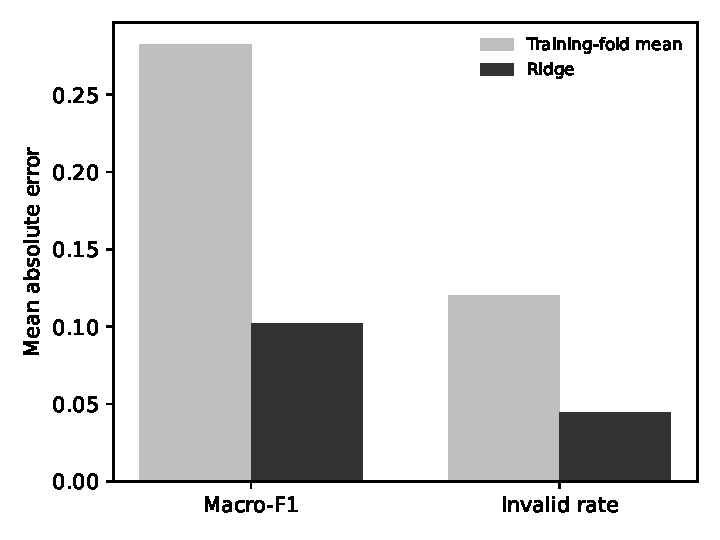
\includegraphics[width=0.72\linewidth]{figures/figure5_esci.pdf}
\caption{ESCI only. Macro-F1 error is 0.2825 for the training-fold mean and 0.1024 for ridge. Invalid-rate error is 0.1199 and 0.0444. Both predictors and the oracle select the classifier.}
\label{fig:esci}
\end{figure}
\FloatBarrier

\subsection{Generative validity}
\label{sec:validity}

\Cref{tab:validity} is the main validity result. The rule, the classifier, and Laya produce no invalid outputs. Qwen's invalid-output rate varies substantially across tasks.

On Civil Comments every one of the 1{,}000 outputs is invalid, so macro-F1 is 0. That zero is a measured contract failure, not a hand-entered score. On Banking77 and CLINC150 plus, invalid outputs are 514 and 745 of 1{,}000 rows, so the resulting macro-F1 is strongly affected by output validity. On SMS Spam, VitaminC, and ESCI, invalid outputs are 25, 23, and 32 of 1{,}000 rows. Macro-F1 on those tasks is mostly the legal predictions, and it is still low relative to the classifier (0.2067, 0.2209, and 0.0358).

The raw strings that failed the match were not saved. We cannot say whether they were explanations, extra words, or misspelled labels. We can establish only that they did not satisfy the exact legal-label criterion defined by the frozen protocol. A future experiment could retain the invalid strings to distinguish formatting, explanation, spelling, and other failure modes. Changing the prompt, the decoder, or the parser to reduce \(V\) would be a different primitive.
